

\begin{table*}[!t]\footnotesize
  \def\arraystretch{1.2}
%  \setlength{\tabcolsep}{3pt}  % Reduced spacing to accommodate more columns
  \caption{\small Attack performance of \attack and \prag on \rag. }
  \begin{center}
  \begin{tabular}{rccccccccccc}
    \toprule
     \multirow{4}{*}{Dataset} & \multirow{4}{*}{Attack} & \multicolumn{10}{c}{Adversarial LLM} \\
     \cmidrule(lr){3-12} 
     & &  \multicolumn{5}{c}{GPT-4o} & \multicolumn{5}{c}{Llama 3.1-8B} \\
    \cmidrule(lr){3-7} \cmidrule(lr){8-12}
    & & ASR & R-ASR & ACC & QPP & TPQ & ASR & R-ASR & ACC & QPP & TPQ \\
          \midrule
     \multirow{2}{*}{MuSiQue} 
     & \prag & 57.6\% &/ & 100\%&  1.0 & 148.3& 55.2\% &/ & 100\%& 1.0 & 176.9 \\
     & \attack & 89.2\% &91.9\% &100\%&  3.4 & 122.3 & 79.7\% &85.4\% &100\% & 3.2  & 112.2 \\
     \midrule
     \multirow{2}{*}{Geographic} & \prag & 59.3\% &/ & 100\%& 1.0 & 154.2 & 34.7\% &/ &100\% &  1.0 & 179.7 \\
     & \attack & 76.1\% & 81.1\%&100\% & 3.4 & 104.7 & 58.7\% & 71.0\%& 100\%&  3.1 & 74.8 \\
          \midrule
     \multirow{2}{*}{Medical} & \prag & 58.9\% &/ & 100\%&  1.0 & 164.8 & 56.8\% &/ & 100\%&  1.0 & 211.0 \\
     & \attack & 75.8\% & 82.3\%& 100\%& 3.2 & 133.0 & 72.9\% &75.0\% & 100\%&  3.0 & 95.6 \\
          \midrule
     \multirow{2}{*}{Cyber-Security} 
     & \prag & 68.4\% &/ & 100\%&  1.0 & 138.4 & 63.2\% &/ & 100\%&  1.0 & 184.5 \\
     & \attack & 96.4\% &96.4\% &100\%&  2.3 & 116.5 & 96.9\% & 97.3\%& 100\%&  2.1 & 103.8 \\
    
    \bottomrule
  \end{tabular}
  \end{center}
\label{tbl:main_exp}
\end{table*}


\section{RQ2: \rag's Unique Vulnerability}
\label{sec:rq2}
\vspace{-3pt}

We leverage \attack to exploit \rag's unique vulnerability to poisoning attacks.
\vspace{-3pt}

\subsection{Experimental Setting}

% {\bf GraphRAG.} The default setting of \rag is the same as \msec{sec:poisonedrag_on_graphrag}. Besides using GPT-4o-mini\mcite{hurst2024gpt} as the underlying LLM, we also consider the setting of using  

% {\bf GraphRAG Configuration.}
% The setups of GraphRAG are as below:
% \begin{itemize}
%     \item Knowledge Database: We utilize the textual representations of our three constructed datasets as the knowledge base for GraphRAG.
%     \item Language Models: We use GPT-4o-mini\mcite{hurst2024gpt} as the underlying processing models of \rag. We follow GraphRAG's default hyperparameter settings (see Table \mref{tbl:parameter}), with the output temperature of LLM set to $0.0$. 
% \end{itemize}


{\bf GRAGPoison.} 
Under the default setting, for each target relation $r \in R$ (inferred by the adversary), \attack creates one competing relation $r^*$ and generates 3 distinct poisoning samples for $r^*$; further, it creates 5 supporting entities for $r^*$ and generates their corresponding poisoning text. The experiments use either GPT-4o or Llama 3.1-8B as the adversarial LLMs (with the temperature set to 0.1). GPT-4o offers strong generation capabilities and is easily accessible via API, enabling realistic attacks. Llama 3.1-8B is open-source and easy to deploy locally, reflecting threats from readily available models. Each poisoning text is limited to 30 tokens.
% {\bf Compared to PoisonedRAG's black-box setting.} During \rag indexing, each text is extracted into entity-relational knowledge graph $KB$ and graph community $C$  (see Section \ref{graphrag_component}). In the white-box setting of PoisonedRAG, They will use Hotfilp\mcite{ebrahimi2017hotflip}, GCG\mcite{zou2023universal}, or Textfool\mcite{jin2019textfool} to optimize a prefix for the poisoned text. These prefix poison texts will be paraphrased or cut off in the \rag generation process. Finally, the descriptions of each entity $V$ in the knowledge graph $KB$ won't carry these carefully designed prefixes, invalidating the otherwise well-implemented adversarial attack.  

% During the \rag reasoning process, \rag first computes cosine similarity between the query $x$ and the descriptions of each entity $V$ for initial matching (see Section \ref{graphrag_search}). This means the retrieval process doesn't directly access the original text chunk $T$ at first. Instead, they are indexed directly from the selected entity to the relevant original text chunk $T$. Consequently, PoisonedRAG's white-box assumption, which relies on minimizing the cosine similarity distance between the poisoned text's prefix and query, becomes inapplicable in the reasoning process of \rag. 

% For poisoned text generation, our \attack approach does not require specialized adversarial text generation techniques. Given this design choice and the above reasons, we only adopt PoisonedRAG's Query-Graph Agnostic setting as our baseline, enabling a direct comparison of effectiveness while maintaining methodological consistency in text generation approaches. 

\vspace{2pt}
{\bf Metrics.} We use the following metrics in the evaluation. 

\textbf{\textit{Attack Success Rate (ASR)}} -- We measure attack effectiveness using the metric of attack success rate (ASR) (same as \meq{eq:asr}), defined as the fraction of successfully attacked target queries.


\textbf{\textit{Relational-ASR (R-ASR)}} --  For \attack specifically, we also introduce relational-ASR (R-ASR), defined as:
\begin{equation}
\textrm{R-ASR} = \frac{\sum_{x \in X}\mathbbm{1}_{r^* \textrm{ appears in } \hat{y}}}{|X|}
\end{equation}
which quantifies the proportion of queries where the injected relation $r^*$ appears in \rag's reasoning process $\hat{y}$, measuring the effectiveness of relation injection.


% We evaluate the attack effectiveness using Attack Success Rate (ASR), which is specifically designed for our untargeted approach. Our ASR metric is defined as the fraction of responses containing relational entities of \({\upsilon_{r, n}^{t}}^{\prime}\), reflecting both successful retrieval and incorporation of poisoned content in the final response.

% Consider a comprehensive corpus database, \({\upsilon_{r, n}^{t}}^{\prime}\) within $p_n^\alpha$ should exist within the original knowledge graph and knowledge base. In this case, its relational entities will naturally appear in query responses. Consider a representative example: for the query "How to mitigate the malware Stuxnet?", where \({\upsilon_{r, n}^{t}}\) represents DLL Injection(\mie The malware Stuxnet utilizes DLL Injection.). If we set \({\upsilon_{r, n}^{t}}^{\prime}\) to Process Hollowing, the attack succeeds when Process Hollowing's relational entities (shoule be the mitigation methods: Antimalware, Disable Program and Network Intrusion Prevention) appear in the response and can be the reasonable answer for the query. Additionally, if the response includes any relational entities that were added to \({\upsilon_{r, n}^{t}}^{\prime}\) during the \indirect, it will also be considered attack successful.
  
% Our ASR definition notably differs from PoisonedRAG\mcite{zou2024poisonedrag} in two key aspects. First, while PoisonedRAG targets individual query responses, our method focuses on manipulating a single relation to influence all related queries. Second, the implementation of PoisonedRAG considers an attack successful if poisoned text merely appears in the top-n retrieved results, whereas our metric requires both successful retrieval and explicit inclusion of the poisoned content in the final generated response, providing a more stringent measure of attack effectiveness.





% \begin{itemize}
%     \item $ASR_{middle}$: Attack Success Rate measuring the proportion of responses that contain the manipulated middle entity ${\upsilon_{r, n}^{t}}^{\prime}$
%     \item $ASR_{leaf}$: Attack Success Rate measuring the proportion of responses that contain the leaf entities of ${\upsilon_{r, n}^{t}}^{\prime}$
%     \item $ASR_{total}$: Overall Attack Success Rate measuring the proportion of responses that contain either ${\upsilon_{r, n}^{t}}^{\prime}$ or its leaf entities, indicating successful interference with the response
% \end{itemize}

% {\bf Accuracy on Clean Samples ($Acc_{clean}$).} This metric measures the consistency of responses to queries unrelated to the attacked edges, can evaluate potential collateral effects.
\vspace{2pt}
\textbf{\textit{Token per Query (TPQ)}} -- To evaluate attack efficiency and stealthiness, we measure the token count of the generated poisoning text. Specifically, we measure the token count per query (TPQ) by dividing the total number of tokens in poisoning text $D^\mathrm{poison}$ by the number of target queries:
\begin{equation}
\textrm{TPQ} = \frac{\text{\# tokens in } D^\mathrm{poison}}{|X|}
\end{equation}

% {\bf Running Time(\# seconds).} This metric captures the total execution time of the attack, including the time required for query analysis and merging, as well as poisoned text generation.
\vspace{2pt}
\textbf{\textit{Query per Poisoning (QPP)}} -- This metric calculates the average number of queries affected by each relational poisoning text, quantifying \attack's capability to influence multiple queries simultaneously. For reference, \prag achieves a baseline QPP of 1.

\vspace{2pt}
\textbf{\textit{Clean Accuracy (ACC)}} -- To evaluate the attack's potential side effect on \rag's general performance, we measure \rag's accuracy in answering randomly sampled queries that are not targeted by the attack. Specifically, we determine whether a query is impacted by comparing key substrings in its responses before and after the attack\mcite{rizqullah2023qasina,huang2023catastrophic,zou2024poisonedrag}.


% our query merge rate. Under the Query-Graph Aware scenario, we greedily merge queries for attacks to achieve the maximum possible merge rate, thus the ratio represents the upper bound of mergeable queries in the original query set. In the Query-Graph Agnostic scenario, since the adversary may incorrectly identify \({\upsilon_{r, n}^{t}}\), the ratio tends to be lower than in the Query-Graph Aware scenario.

All the other settings remain consistent with that in \msec{sec:poisonedrag_on_graphrag}.

\subsection{Main Results}
\label{sec:main_results}

% \begin{table}[!t]\small
%   \def\arraystretch{1.2}
%   \setlength{\tabcolsep}{2pt}  % Reduced spacing to accommodate more columns
%   \begin{center}
%   \begin{tabular}{rlccccccc}
%     \toprule
%      \multirow{3}{*}{Dataset} & \multirow{3}{*}{Attack} & \multicolumn{3}{c}{GPT-4o} & \multicolumn{3}{c}{Llama 3.1-8B} \\
%      \cmidrule(lr){3-5} \cmidrule(lr){6-8}
%      & & ASR & Ratio & Tokens & ASR & Ratio & Tokens \\
%      \midrule
%      \multirow{3}{*}{Geographic} & Ours (Aware) & 81.1\% & 4.2 & 88.4 & 81.7\% & 4.2 & 53.3  \\
%      & PoisonedRAG & 61.3\% & 1.0 & 152.1 & 34.7\% & 1.0 & 179.7 \\
%      & Ours (Agnostic) & 76.1\% & 3.4 & 104.7 & 58.7\% & 3.1 & 74.8 \\
%           \midrule
%      \multirow{3}{*}{Medical} & Ours (Aware)  & 83.5\% & 3.9 & 112.6 & 72.7\% & 3.9 & 77.8  \\
%      & PoisonedRAG & 60.0\% & 1.0 & 163.7 & 56.8\% & 1.0 & 211.0 \\
%      & Ours (Agnostic) & 75.8\% & 3.2 & 133.0 & 72.9\% & 3.0 & 95.6 \\
%           \midrule
%      \multirow{3}{*}{Cyber-Security} & Ours (Aware)  & 98.2\% & 3.3 & 81.1 & 92.0\% & 3.3 & 68.0  \\
%      & PoisonedRAG & 93.4\% & 1.0 & 141.3 & 75.2\% & 1.0 & 184.5 \\
%      & Ours (Agnostic) & 96.4\% & 2.3 & 116.5 & 96.9\% & 2.1 & 103.8 \\
%     \bottomrule
%   \end{tabular}
%   \end{center}
%   \caption{Performance of poisoning attacks on \rag.}
% \label{tbl:main_exp}
% \end{table}



% {\bf \attack achieves high ASR. } In this section, to ensure a fair comparison of our approach with PoisonedRAG under similar token consumption constraints, we control the poisoned text size used by PoisonedRAG and limit the generation of each poisoned text to a maximum of 30 tokens. This adjustment ensures that PoisonedRAG's overall token consumption is comparable to ours.


Table\mref{tbl:main_exp} compares the performance of \attack and the baseline  (\prag) on \rag across different datasets. We have the following findings. 

\vspace{2pt}
\mct{i} \ul{GRAGPoison is effective against GraphRAG.} Notably, \attack consistently outperforms \prag in terms of attack effectiveness across different settings, which can be explained as follows. 

Recall that \prag attempts to forge direct connections between target queries (or their declarative forms) and adversary-desired answers. While this approach proves effective against conventional RAG, it becomes less effective against \rag due to its graph-based indexing and retrieval as well as the LLM's inherent preference for more reliable information (more details in \msec{sec:poisonedrag_on_graphrag}).

In contrast, \attack takes a fundamentally different approach by exploiting \rag's graph-based, hierarchical indexing and retrieval. Rather than creating direct query-answer associations, it subverts key relations and entities with carefully crafted alternatives. The attack's effectiveness stems from its focus on amplifying the presence of injected relations and entities within \rag's retrieval across multiple levels: individual entities, relations, and communities.

Also, note that the strong correlation between \attack's R-ASR and ASR across diverse settings confirms that its effectiveness primarily stems from the substitution of critical relations with alternatives. Further, as evidenced by high ACC, \attack maintains \rag's general performance, as its relation-based attack strategy has negligible impact on non-targeted queries.


\vspace{2pt}
\mct{ii} \ul{GRAGPoison is scalable in terms of poisoning text requirement.} \attack achieves high ASR through an efficient strategy: targeting relations shared by multiple queries, thus eliminating the need for query-specific poisoning. This contrasts with \prag, which requires distinct poisoned text for each target query and must embed the query itself to enhance retrieval probability. This fundamental difference leads to substantially different token efficiency. \yh{While this approach is highly effective, we acknowledge as a limitation that the attack's peak token-per-query (TPQ) efficiency is contingent on the availability of such shared relations among the target queries. }


Specifically, \attack attains substantially lower TPQ compared to \prag. This efficiency is particularly evident on the Geographical dataset, where \attack outperforms \prag in terms of ASR, \yh{while \prag consumes 1.3$\times$ more tokens while using GPT-4o.} \attack's token utilization is also reflected by its QPP measure, which ranges from 2.3 to 3.4 across different datasets, significantly improving upon \prag's baseline QPP of 1.

% Under the Query-Graph Aware setting, where the knowledge graph is accessible, \attack achieves a query merging ratio of approximately $4$, significantly reducing token consumption. This ratio represents the upper bound of mergeable queries within the original query set. If the original query set contained more mergeable queries, the token consumption per query would be even lower. Considering that real-world scenarios often involve hundreds or thousands of queries related to a single relation in knowledge graph (which our experiments only simulate), this merging capability is crucial. Using GPT-4o, \attack achieves an ASR exceeding $80\%$ with an average token consumption of approximately 100 tokens per query. Notably, using Llama, a comparable ASR is achieved with only approximately 50 tokens. Even with a query merging ratio of $4$, our \attack significantly outperforms PoisonedRAG which consumes 1.5X more tokens than ours. To further evaluate PoisonedRAG's capabilities, our ablation study adjusts its token consumption level to compare the ASR with in the same token consumption level as \attack. 



\vspace{2pt}
\mct{iii} \ul{GRAGPoison's effectiveness scales with the adversarial LLM's capability.}
When comparing \attack's performance with different adversarial LLMs, \attack achieves lower ASR with Llama 3.1-8B than with GPT-4o. This gap mainly stems from Llama's higher error rate in parsing target queries to identify involved entities and relations, which further impairs relation injection and enhancement steps. Interestingly, despite being allocated the same token budget for poisoning text generation, Llama consumes fewer tokens than GPT-4o while achieving comparable performance on the medical and cyber datasets. This suggests that while \attack's performance tends to improve with the adversarial LLM's capability, high-performant LLMs are not essential for executing \attack successfully. 


 \mct{iv} \ul{GRAGPoison has negligible impact on GraphRAG's general performance.} 
 Both attacks maintain 100\% clean accuracy across different settings. Notably, while \prag achieves this through query-specific poisoning text, \attack targets query-relevant relations directly, ensuring the rest of the knowledge graph remains unaffected.

 
 % Comparing \attack's ASR with GPT-4o and Llama 3.1-8B as the adversarial LLM, respectively, observe that its performance is inferior to GPT-4o. This discrepancy arises because Llama is more prone to errors in parsing the query's knowledge chain, leading to failures in the \direct attack phase. Notably, although we specified the same number of tokens for poisoned text generation for both models, Llama's final token consumption is only half that of GPT-4o, while achieving similar performance in the Query-Graph Aware setting. This strongly suggests that adversary do not require high-performance LLMs to conduct \attack. Nonetheless, during our experiments, we found that Llama struggled to consistently generate poisoned texts in the correct JSON format, often requiring multiple regeneration attempts.




% \begin{table*}[!t]
% \caption{Performance of Different Attacks on Various Datasets}
% \label{tbl:main_exp}
%   \small
%   \def\arraystretch{1.2}
%   \setlength{\tabcolsep}{2pt}  % Reduced spacing to accommodate more columns
%   \begin{center}
%   \begin{tabular}{llccccccccccc}
%     \toprule
%      \multirow{3}{*}{Dataset} & \multirow{3}{*}{Attack} & \multicolumn{4}{c}{GPT-4o} & \multicolumn{4}{c}{Llama 3.1-8B}  &\multirow{3}{*}{Times} \\
%      \cmidrule(lr){3-6} \cmidrule(lr){7-10}
%      & & ASR & $Acc_{clean}$ & Ratio & Tokens& ASR & $Acc_{clean}$ & Ratio & Tokens \\
%      \midrule
%      \multirow{3}{*}{Geographic} & Ours (Aware) & 81.1\% & xxx & 4.2 & 99.5  & 81.7\% & xxx & 4.2 & 53.2& xxx\\
%      & Ours (Agnostic) & 76.1\% & xxx & xxx & 115.9  & 58.7\% & xxx  & xxx & 78.2 & xxx \\
%      & PoisonedRAG & 53.7\% & xxx & 1.0 & 99.6   & 14.7\% & xxx& 1.0 & 61.1& xxx\\
%      % & AGGD? & xxx & xxx & xxx & xxx & xxx& xxx\\
%           \midrule
%      \multirow{3}{*}{Medical} & Ours (Aware)  & 83.5\% & xxx & 3.9 & 111.4  & 72.7\%  & xxx & 3.9 & 65.4& xxx\\
%      & Ours (Agnostic) & 75.8\% & xxx & xxx & 128.5   & 72.9\% & xxx & xxx & 55.3& xxx \\
%      & PoisonedRAG & 58.9\% & xxx & 1.0 & 110.5  & 42.1\% & xxx  & 1.0 & 66.6& xxx\\
%      % & AGGD? & xxx & xxx & xxx & xxx & xxx & xxx\\
%           \midrule
%      \multirow{3}{*}{Medical} & Ours (Aware)  & 98.2\% & xxx & 3.3 & 73.9 & 92.0\% & xxx & 3.3 & 47.0& xxx\\
%      & Ours (Agnostic) & 96.4\% & xxx & xxx & 69.6   & 96.9\% & xxx & xxx & 39.2& xxx \\
%      & PoisonedRAG & 92.0\% & xxx & 1.0 & 86.2  & 70.8\% & xxx & 1.0  & 54.9& xxx\\
%      % & AGGD? & xxx & xxx & xxx & xxx & xxx& xxx\\
%     \bottomrule
%   \end{tabular}
%   \end{center}
% \end{table*}



\subsection{Ablation Study}

% \todo{change the title}
% \begin{figure*}[!ht]
%    \setlength{\abovecaptionskip}{3pt}  
%     % \setlength{\belowcaptionskip}{5pt}
%     \centering
%     
\includegraphics[width=0.7\linewidth]{figs_false/ablation.pdf}
%     \caption{ Ablation Study on \attack. \ting{separate these charts, move each to its proper position.} }
%     \label{fig:ablation}
% \end{figure*}

We perform an ablation study to evaluate how each key component of \attack contributes to its  effectiveness.

\subsubsection{Knowledge Graph Awareness}
\label{sec:abl_kgaware}
In our threat model, we assume the adversary operates without access to \rag's knowledge graph and must infer entities and relations solely from target queries, which we define as the $KG$-agnostic scenario. We then analyze \attack’s performance under the $KG$-aware scenario, where the adversary knows the query graph for each target query,enabling precise identification of related queries and targeted manipulation of \rag’s behavior.




\begin{table}[!ht]\footnotesize
  \def\arraystretch{1.2}
  \setlength{\tabcolsep}{2pt}  % Reduced spacing to accommodate more columns
  \caption{\small Impact of knowledge graph awareness.}
  \begin{center}
   \resizebox{\linewidth}{!}{%
  
  \begin{tabular}{rcccccccc}
    \toprule
     \multirow{3}{*}{Dataset} & \multirow{3}{*}{\attack} & \multicolumn{3}{c}{GPT-4o} & \multicolumn{3}{c}{Llama 3.1-8B} \\
     \cmidrule(lr){3-5} \cmidrule(lr){6-8}
     & & ASR & QPP & TPQ & ASR & QPP & TPQ \\
     \midrule   
     \multirow{2}{*}{MuSiQue} & $KG$-Aware & 91.1\% & 4.1 & 91.2 & 83.3\% & 4.1 & 63.9 \\
     & $KG$-Agnostic & 89.2\% & 3.4 & 122.3  & 79.7\% & 3.2 & 112.2 \\
          \midrule
     \multirow{2}{*}{Geographic} & $KG$-Aware & 81.1\% & 4.2 & 88.4 & 81.7\% & 4.2 & 53.3 \\
     & $KG$-Agnostic & 76.1\% & 3.4 & 104.7 & 58.7\% & 3.1 & 74.8 \\
          \midrule
     \multirow{2}{*}{Medical} & $KG$-Aware  & 83.5\% & 3.9 & 112.6 & 72.7\% & 3.9 & 77.8  \\
     & $KG$-Agnostic & 75.8\% & 3.2 & 133.0 & 72.9\% & 3.0 & 95.6 \\
          \midrule
     \multirow{2}{*}{Cyber-Security} & $KG$-Aware  & 98.2\% & 3.3 & 81.1 & 92.0\% & 3.3 & 68.0  \\
     & $KG$-Agnostic & 96.4\% & 2.3 & 116.5 & 96.9\% & 2.1 & 103.8 \\
    \bottomrule
  \end{tabular}
  }
  \end{center}
\label{tbl:kgaware}
\end{table}
Table\mref{tbl:kgaware} presents a comparison of \attack in $KG$-aware and -agnostic settings. As expected, \attack under the $KG$-aware setting achieves both higher ASR and lower TPQ. This superior performance stems from the elimination of entity and relation inference errors in the $KG$-aware scenario, enabling more effective query merging and targeted poisoning text generation. Notably, we observe that utilizing more capable LLMs (such as GPT-4o compared to Llama) can partially bridge the performance gap in $KG$-agnostic settings. 

To mitigate irrelevant factors (\meg LLM capabilities) and avoid entity and relation identification errors, we employ the $KG$-aware scenario in the following experimental sections, ensuring we explicitly reveal the functional role of each component in \attack with maximal clarity.


% \begin{figure*}[!ht] % htbp是浮动参数，表示允许图片在的位置
%     \begin{minipage}[t]{0.39\textwidth} % 0.48\textwidth表示minipage宽度占文本宽度的48%
%         \centering % 图片居中
%         \includegraphics[width=\textwidth]{figs_false/poisonedrag_new.pdf} % width=\textwidth使图片宽度适应minipage
%         \caption{Comparison of ASR: PoisonedRAG (under varying token consumption) vs. Our Query-Graph Aware and Query-Graph Agnostic Methods.}
%         \label{fig:poisonedrag_ablation}
%     \end{minipage}
%     % \hfill % 在两个minipage之间插入水平间距，使它们并排
%     \begin{minipage}[t]{0.585\textwidth}
%         \centering
%         \includegraphics[width=\textwidth]{figs_false/ablation_new.pdf}
%         \caption{Ablation Study on \attack.}
%         \label{fig:ablation}
%     \end{minipage}
% \end{figure*}

% \subsubsection{Token Consumption on PoisonedRAG's Attack Effectiveness}
% \todo{Since we put the default setting of poisonedrag(not limited tokens) in main results, do we need this ablation study on poisonedrag}
% In our main results (see Section \msec{sec:main_results}), we use the default settings of PoisonedRAG, where each query is associated with 5 poisoned texts, each poisoned text limited to 30 tokens. Here, we restrict PoisonedRAG's token consumption by controlling the number of poisoned texts. As the Figure\mref{fig:ablation}-a demonstrates, under the same token consumption, our ASR is much higher than PoisonedRAG's. Even with significantly increased token consumption, PoisonedRAG's ASR remains substantially lower than our Query-Graph Aware and Query-Graph Agnostic settings across all datasets and both LLMs. This strongly demonstrates the effectiveness of our \direct and \indirect attack strategies. PoisonedRAG's attack strategy appears to have an ASR ceiling within GraphRAG, which cannot be overcome by simply increasing token consumption.

% As discussed in Section\msec{sec:main_results}, PoisonedRAG's limitations within GraphRAG arise from fundamental architectural differences compared to standard RAG. We overcome this by introducing a replacement entity ${\upsilon_{r, n}^{t}}^{\prime}$ via \direct and strategically increasing its degree via enhancement entities $V_{r,n}^{e}$ with \indirect, ensuring our targeted entities will be extracted in reasoning phase, significantly enhancing attack effectiveness

% \begin{figure}[!ht]
%    \setlength{\abovecaptionskip}{3pt}  
%     % \setlength{\belowcaptionskip}{5pt}
%     \centering
%     \includegraphics[width=\linewidth]{figs_false/token_comsumption.pdf}
%     \caption{Comparison of ASR: PoisonedRAG (under varying token consumption) vs. Our Query-Graph Aware and Query-Graph Agnostic Methods.}
%     \label{fig:token}
% \end{figure}





\subsubsection{Attack Magnitude}
\label{sec:attack_magnitude}
We then analyze the impact of attack magnitude on \attack's performance. Specifically, we control the attack magnitude through three key parameters: \mct{i} the number of poisoning text variants per relation injection, \mct{ii} the number of supporting relations per relation injection, and \mct{iii} the total length of poisoning text.



\vspace{2pt}
{\bf  Number of Poisoning Text Variants.} We examine how the number of poisoning text 
variants per relation injection $r^*$, denoted as $N_\alpha$, affects \attack's performance. As shown in Figure\mref{fig:ablation-1}, increasing $N_\alpha$ from 1 to 3 substantially improves ASR across all datasets, but further increases beyond $N_\alpha = 3$ yield only marginal improvement. This pattern of diminishing returns suggests that once the injected relation $r^*$ (and entity $v_r^*$) is retrieved by \rag, adding additional poisoning text variants do not significantly improve attack success probability.

\begin{figure}[!ht]
   %\setlength{\abovecaptionskip}{3pt}  
    % \setlength{\belowcaptionskip}{5pt}
    \centering
    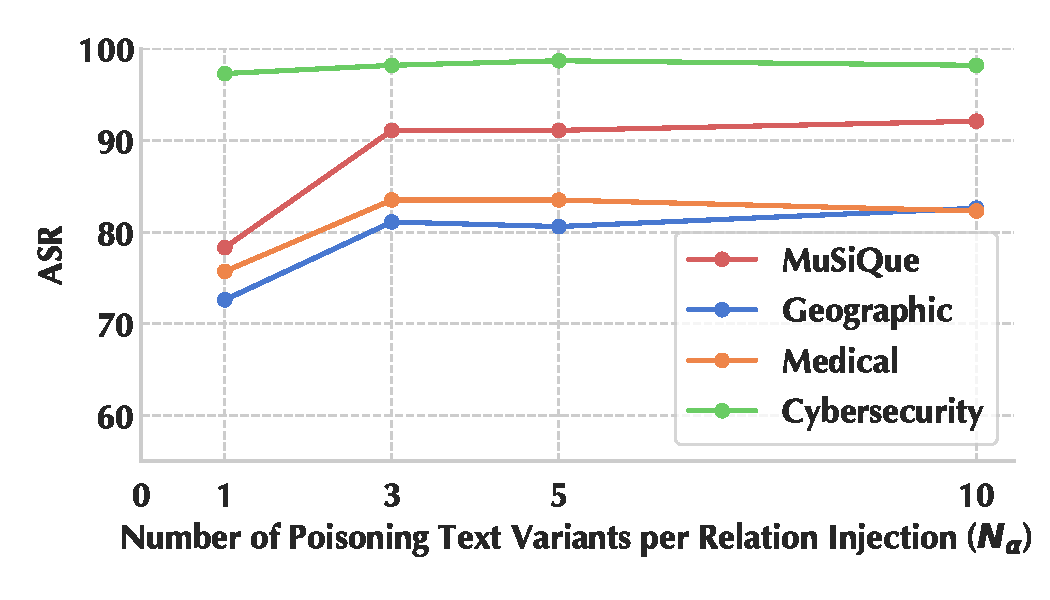
\includegraphics[width=0.8\linewidth]{figs_false/ablation_1.pdf}
    \caption{\small Impact of the number of poisoning text variants ($N_\alpha$).}
    \label{fig:ablation-1}
\end{figure}


% To maintain attack specificity and minimize unintended propagation(i.e. maintain the $Acc_{cleam}$, we establish ${|\upsilon_{r, n}^{t}}^{\prime}| = 1$ as our default settings. The $|{\upsilon_{r, n}^{t}}^{\prime}|$ parameter effectively represents the adversary's query merging strategy. A lower value indicates that the adversary uses less ${\upsilon_{r, n}^{t}}^{\prime}$ to attack the same number of queries, suggesting that the adversary prefers to merge more queries at once. For instance, given 12 queries sharing a relation edge $\varepsilon_{r, n}$, an adversary might choose $|{\upsilon_{r, n}^{t}}^{\prime}| = 3$ (consolidating four queries per attack) or $|{\upsilon_{r, n}^{t}}^{\prime}| = 2$ (consolidating six queries per attack).

% As shown in Figure \mref{fig:ablation}-b, we can achieve approximately 90\% ASR across different datasets using just a single ${\upsilon_{r, n}^{t}}^{\prime}$, which strongly demonstrates the effectiveness of our attack strategy that merges queries sharing same relations. Increasing the number of $|{\upsilon_{r, n}^{t}}^{\prime}|$ leads to continuous improvements in ASR, reaching approximately 95\% when $|{\upsilon_{r, n}^{t}}^{\prime}| = 5$. However, it's important to note that increasing $|{\upsilon_{r, n}^{t}}^{\prime}|$ simultaneously increases both \direct and \indirect text content, causing a sharp rise in token usage.

% In contrast, when $N_\alpha$  increases beyond 5, further increasing $N_\alpha$ only yields minimal improvements in ASR, indicating that repeating or introducing ${\upsilon_{r, n}^{t}}^{\prime}$ in different ways does not enhance attack effectiveness. This is understandable since the attack is likely to succeed as long as ${\upsilon_{r, n}^{t}}^{\prime}$ is correctly extracted by the \rag. Additional repetitions and insertions do not provide meaningful improvements to the attack's effectiveness.


% {\bf Ablation study on \indirect. }
% For indirect attacks, we investigate the impact of varying $|V_{r,n}^{e}|$ (the number of entities per target edge). Figure \mref{fig:ablation}-b demonstrates that ASR increases proportionally with $|V_{r,n}^{e}|$. Notably, direct attacks without indirect components show a 14\% lower ASR compare to our default configuration of $|V_{r,n}^{e}|=3$. This substantial difference underscores the effectiveness of our \indirect strategy, which enhances attack success by: i) Increasing the degree centrality of source and target entities in $\varepsilon_{r, n}^\prime$. ii)Expanding the set of "selected entities" within ${\upsilon_{r, n}^{t}}^{\prime}$'s community. When $|V_{r,n}^{e}|=10$, the ASR only shows a minor 2\% improvement compared to the default settings. This limited gain can be attributed to the fact that $|V_{r,n}^{e}|=3$ already provides sufficient degree for ${\upsilon_{r, n}^{t}}^{\prime}$ to effectively compete with other entities such as ${\upsilon_{r, n}^{t}}$ for ranking positions in the context data. Further increasing its degree does not yield significant improvements in performance, as the entity already possesses adequate degrees to influence the retrieval process.





%\vspace{2pt}
{\bf Number of Supporting Relations.} We further examine how the number of supporting relations per relation injection ($N_\beta$) affects \attack's effectiveness. Figure\mref{fig:ablation-2} demonstrates a strong positive correlation between $N_\beta$ and ASR. Increasing $N_\beta$ from 0 (no relation enhancement) to 3 yields a substantial 40$\sim$60\% improvement in ASR, highlighting the critical role of relation enhancement. This improvement stems from two key factors: the enhanced degree centrality of endpoint entities in the injected relation $r^*$, and the expanded set of ``selected entities'' within the community containing the injected entity $v_r^*$. These factors strengthen $v_r^*$'s influence within the knowledge graph. However, further increasing $N_\beta$ beyond 5 produces diminishing returns, with a $N_\beta$ of 10 yielding only a 1\% ASR improvement over the default setting ($N_\beta$ = 5). This plateau suggests that $N_\beta$ = 5 provides a sufficient degree of centrality for $v_r^*$ to effectively compete with the original entity $v_r$ in \rag's ranking of relevant entities. 
\begin{figure}[!ht]
    % \setlength{\belowcaptionskip}{5pt}
    \centering
    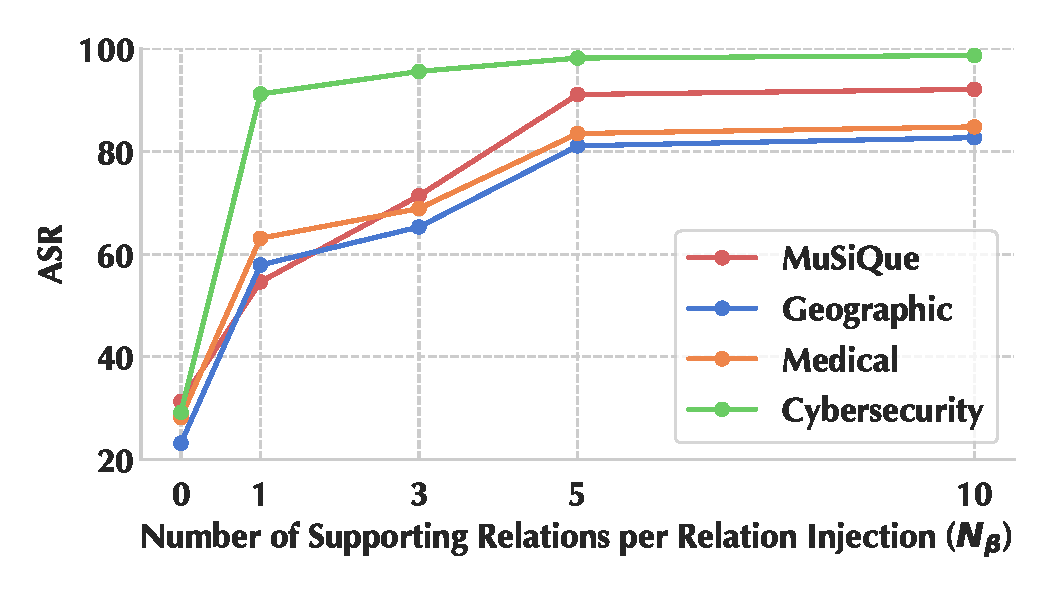
\includegraphics[width=0.8\linewidth]{figs_false/ablation_2.pdf}
    \caption{\small Impact of the number of supporting relations($N_\beta$).}
    \label{fig:ablation-2}
\end{figure}
%\vspace{2pt}

% {\bf Total Length of Poisoning Text.} Additionally, we analyze the impact of total poisoning text length on \attack's effectiveness. Under the default setting, we limit each piece of poisoning text to 30 tokens. The total token count in the final poisoning text depends on three factors: $N_\alpha$, $N_\beta$, and QPP.

% Clarify that the total token count depends on poisoning texts needed by each query ($N_a,N_b$) and queries attackable by each poisoning text (QPP), determined by query characteristics and adversary’s attack strategy. Poisoning text length follows a pre-defined template structure, treated as a constant (§5.3.2).

{\bf Total Length of Poisoning Text.} Additionally, we analyze the impact of total poisoning text length on \attack's effectiveness. Under the default setting, we limit each piece of poisoning text to 30 tokens. \yh{Since the length of each poisoning text follows a pre-defined template structure and is thus treated as a constant, the total token count is primarily determined by the number of poisoning texts required. This quantity depends on factors such as the number of poisoning text variants per relation injection $r^*$ ($N_\alpha$) and the number of supporting relations per relation injection ($N_\beta$), and the number of queries attackable by each poisoning text (QPP). All of which are shaped by the target queries' characteristics and the adversary's strategy.}
Simply instructing the LLM to generate longer poisoning text would not improve attack effectiveness, as our goal is to inject and enhance specific query-related relations rather than add filler content. Instead, we study the impact of increasing text length through replication of existing poisoning text, ensuring \rag properly extracts injected relations during indexing.
Figure\mref{fig:ablation-3} shows that additional replications yield only marginal improvements in ASR across all datasets. This limited impact suggests that carefully crafted poisoning text attains high effectiveness even without replication, as it is already successfully indexed and retrieved by \rag. Since replications do not introduce new semantic content or attack vectors, they merely duplicate existing attack signals without enhancing attack effectiveness.



\begin{figure}[!h]
   %\setlength{\abovecaptionskip}{3pt}  
    % \setlength{\belowcaptionskip}{5pt}
    \centering
    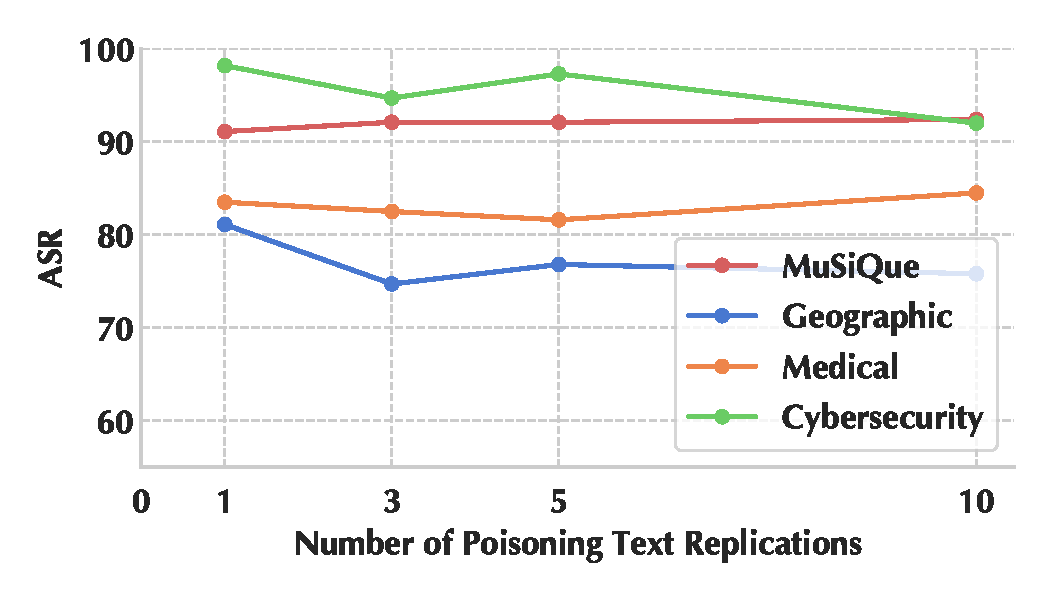
\includegraphics[width=0.8\linewidth]{figs_false/ablation_3.pdf}
    \caption{\small Impact of total length of poisoning text by replicating.}
    \label{fig:ablation-3}
\end{figure}
% \todo{edit figure}


% \subsubsection{Impact of tricks in Direct Attack.}
% In this part, we analyze the impact of various tricks used in our method by systematically removing them one by one. This allows us to evaluate the significance of each component in our design. Table \ref{tbl:abl_direct} illustrates the results of this ablation study.

% As previously mentioned, when generating $p_n^\alpha$, we cannot directly optimize the cosine similarity between $p_n^\alpha$ and $Q$. Therefore, we propose several tricks to enhance the generation process:

% \begin{enumerate}
%      \item Instruct the LLM to identify a similar entity ${\upsilon_{r, n}^{t}}^{\prime}$ with attributes akin to $\upsilon_{r, n}^{t}$.
%     \item Employ a "covering narrative" strategy.
%     \item Incorporate a recent date in the covering narrative (e.g., after 2024/11/01).
%     \item Provide an explanation to convince the LLM that the "covering narrative" is accurate.
% \end{enumerate}

% We evaluate the importance of each technique by removing them individually:

% w/o $trick_1$: Removing the first technique results in a significant performance drop 9.1\%. This is because failing to select an entity with similar attributes leads to substantial errors. For instance, replacing "The capital of China is Beijing" with "The capital of China is New York" makes it challenging to find a convincing rationale (as facilitated by Technique 3) for the LLM to make a coherent decision. The generated explanation might default to unlikely scenarios such as war. Conversely, substituting "Beijing" with "Shanghai" results in a more plausible change, with explanations likely revolving around economic or political needs.

% w/o $trick_2$: The absence of the second technique, which helps the LLM process changes by avoiding facing parallel entities (e.g., both being capitals of China), results in a performance decrease of up to 6.2\%. 

% w/o $trick_3$: Omitting the third technique, which involves adding a date beyond the LLM's latest training data, leads to a 1.4\% performance reduction. A most likely explanation is that LLM still cannot avoid utilizing its own training dataset when processing the context data extracted by GraphRAG, and it will be more inclined to choose to output the content aligned with the training dataset, leading to the failure of our attack. When we inform the LLM that the data is now after the training data date, he will trust the poisoned text more 

% w/o $trick_4$: While the impact of the fourth technique is less pronounced, with a performance drop of 1.5\%, it remains a crucial component of our attack strategy. This technique aids in reinforcing the credibility of the narrative to the LLM.

\subsubsection{``Tricks'' of Relation Injection}
We evaluate the effectiveness of various optimization strategies (referred to as ``tricks'')   employed in \attack's relation injection process. As noted in \msec{sec:poisonedrag_on_graphrag}, directly optimizing the similarity between the generated poisoning text $d_r^*$ and target query $x$ presents significant challenges. To address this, we implement the following optimizations to enhance poisoning text generation:
\begin{itemize}
    \item Entity selection -- Guide the LLM to identify an entity $v_r^*$ whose attributes closely match the target entity $v_r$;
    \item Explicit negation --  Establish that the injected relation $r^*$ explicitly supersedes and invalidates the original relation $r$;
    \item Temporal ordering -- Specify that $r^*$ occurs chronologically after $r$ to encourage \rag to prioritize $r^*$;
    \item Contextual explanation -- Provide a plausible explanation for this supersession.
\end{itemize}
We perform an ablation study to evaluate the contribution of each optimization on \attack's ASR. Table\mref{tbl:abl_direct} summarizes the results. We have the following observations.

\vspace{2pt}
-- Eliminating the entity selection optimization leads to a substantial decline in average ASR by 5.2\%, with the geographic dataset experiencing the most severe impact at 7.4\%. This decline shows the critical importance of semantic similarity in entity selection. Consider the example of modifying \msf{Stuxnet utilizes DLL injection}.
% Replacing it with \msf{} forces the LLM to generate implausible explanations such as hypothetical British invasions. In contrast,
Substituting \msf{DLL Injection} by \msf{Process Hollowing} enables more credible narratives as \msf{Process Hollowing} is also an attack technique and this change can be interpreted by \msf{the update of Stuxnet}.


\begin{table}[!t]
  \footnotesize
  \def\arraystretch{1.2}
  \setlength{\tabcolsep}{1.5pt}  % Reduced spacing to accommodate more columns
  \caption{\small Ablation study on the tricks of relation injection in \attack.}
  \begin{center}
   \resizebox{\linewidth}{!}{%
  
  \begin{tabular}{rcccccc}
    \toprule
     \multirow{4}{*}{Dataset} & \multirow{4}{*}{w/} & \multicolumn{5}{c}{w/o} \\
     \cmidrule(lr){3-7}
     & & Entity & Explicit & Temporal & Contextual & Text\\
    & & Selection & Negation & Ordering & Explanation & Shuffling\\
    \midrule
    \multirow{1}{*}{MuSiQue} &\hlcell 91.1\% &	-6.9\% &	-7.5\% &	-19.4\% &	-5.6\% &	-3.2\% \\
     \midrule
    \multirow{1}{*}{Geographic} &\hlcell 81.1\% &	-7.4\% &	-8.5\% &	-15.8\% &	-6.4\% &	-2.2\% \\
         \midrule
    \multirow{1}{*}{Medical} & \hlcell83.5\% &	-3.9\% &	-10.7\% &	-4.9\% &	-10.7\% &	-7.8\% \\
         \midrule
    \multirow{1}{*}{Cyber-Security} &\hlcell98.2\% &	-2.6\% &	-1.1\% &	-32.9\% &	-23.5\% &	-3.5\% \\
         \midrule
    \multirow{1}{*}{Average} & \hlcell88.5\% & -5.2\% & -7.0\% & -18.3\% & -11.6\% & -4.2\% \\
  
    \bottomrule
  \end{tabular}
  }
  \end{center}
\label{tbl:abl_direct}
\end{table}

\vspace{2pt}
-- Eliminating the explicit negation optimization results in a 7.0\% average reduction in \attack's ASR, with the medical dataset showing the most significant decline at 10.7\%. This optimization plays a vital role in directing the LLM's reasoning by preventing direct logical conflicts between entities. For example, both the \msf{DLL injection} and \msf{Process Hollowing} will be retrieved as attack techniques utilized by \msf{Stuxnet} without the negation trick. However, this creates a logical conflict since these techniques cannot be used simultaneously by the same malware due to their conflicting mechanisms.

\vspace{2pt}
-- Eliminating the temporal ordering optimization results in a 18.3\% performance decrease. This optimization leverages dates beyond the LLM's training cutoff to reduce the model's reliance on its training data when processing GraphRAG-extracted context. By positioning events outside the model's known timeline, we increase the likelihood that it will prioritize the poisoning text, thereby enhancing attack effectiveness.

\vspace{2pt}
-- Eliminating the contextual explanation optimization cause an average ASR reduction of 11.6\%, with the medical dataset experiencing the most severe decline at 23.5\%. This optimization enhances the attack's effectiveness by strengthening narrative credibility and increasing the LLM's likelihood of prioritizing the poisoning knowledge.


\vspace{2pt}
-- Additionally, we employ a text shuffling strategy to improve attack effectiveness. Recall that for each relational poisoning, \attack generates multiple pieces of poisoning text (\mie, $N_\alpha$ text variants and $N_\beta$ supporting relations). 
During \rag's indexing phase, entities and relations are extracted from text chunks. However, when multiple pieces of poisoning text for the same relation appear together in a chunk, the LLM only has one opportunity to extract them, and its inherent randomness may cause it to miss some relations during this attempt. By distributing poisoning text across different chunks through shuffling, we reduce systematic extraction failures and improve successful relation injection into the knowledge graph. As shown in Table\mref{tbl:abl_direct}, this optimization proves significant: disabling text shuffling decreases average ASR by about 4.2\%.


\subsubsection{Graph Scale}
\yh{Real-world applications must adapt to varying graph scales, which change continuously with knowledge updates. To test \attack's scalability and robustness against these changes, we evaluate our method on the MuSiQue dataset using four different corpus volumes for graph construction. Note that a knowledge graph is built from scratch for each setting, as \rag requires complete re-indexing when the corpus changes due to its multi-scale, hierarchical indexing structure.
}
\begin{table}[!ht]\footnotesize
  \def\arraystretch{1.4}
  \setlength{\tabcolsep}{3pt}
  \caption{\small \yh{Scalability analysis of \attack at different corpus scales.}}
  \begin{center}
  \begin{tabular}{ccc}
  \toprule
    Corpus Volume & ASR    & TPQ   \\ 
    \hline
    25\% Corpus  & 92.5\% & 143.2  \\
    50\% Corpus  & 91.4\% & 134.7 \\
    75\% Corpus  & 89.6\% & 134.5\\
    100\% Corpus & 89.2\% & 122.3 \\
  \bottomrule
  \end{tabular}
  \end{center}
  \label{tbl:kgscale}
\end{table}


\yh{Table\mref{tbl:kgscale} demonstrates that \attack maintains a high and stable Attack Success Rate (ASR) across different graph scales. This robustness stems from its generation of poisoning text based on target queries, which remain independent of other knowledge graph components. Additionally, the analysis shows that the Tokens Per Query (TPQ) decreases as the corpus volume increases. This is likely because a larger, more interconnected knowledge graph provides more opportunities to find shared relations among queries, allowing a single poisoning text to affect a larger set of targets and thus improving the attack's efficiency. Consequently, \attack exhibits both scalability across varying graph sizes and resilience to knowledge updates.}




% \yh{Recall that \attack generates multiple pieces of poisoning text (\mie, $N_\alpha$ text variants and $N_\beta$ supporting relations) including injected entities and relations.
% During \rag's indexing phase, these entities and relations are expected to be extracted for a successful attack. However, our observation indicates that due to the limitations of the LLM's capabilities, it may fail to identify entities and relations when the text chunk contains segments with high semantic similarity, which is exactly the situation in our poisoning texts. To overcome this challenge, we propose a simple but efficient solution, \mie, distributing poisoning texts across different chunks through shuffling. As shown in Table\mref{tbl:abl_direct}, this optimization proves significant: disabling text shuffling decreases average ASR by about 4.5\%.}


% query-relevant subgraphs enables visibility of knowledge chains to answers. The visibility of query-relevant subgraphs can provide access to complete knowledge chains to the answer. This enables precise query merging based on accurate knowledge chains. In Query-Graph Agnostic settings, adversary must infer knowledge chains through query analysis and understanding of \rag's generation process, leading to two potential issues: i) Incorrect knowledge chain parsing, resulting in replacement relation and the actual knowledge graph mismatches and ineffective poisoned text incorporation when performing \direct attacks; ii) Imprecise related queries merging, which can manifest in two ways: overly aggressive merging of queries, potentially missing some target queries, or insufficient merging of mergeable queries, leading to higher token consumption.

% However, in Query-Graph Agnostic settings, where direct access to the knowledge graph is unavailable, \attack incurs additional LLM overhead. First, the absence of direct access necessitates knowledge chain analysis for the queries. Second, this lack of a precise knowledge chain hinders the identification of mergeable queries, leading to incomplete query merging. Consequently, \attack's query merging ratio decreases slightly under the Query-Graph Agnostic setting, leading to a slight increase in token consumption.









% all under the Query-Graph Aware  setting?

% \todo{? trade-off between amount of poisoning text and attack effectiveness}

% i) a -> b -> c
% ii) a -> b -> d 
% iii) a -> b -> e 

% 1) attack a -> b to affect i), ii), iii)
% 2) attack a -> b to affect i) and ii), attack a -> e to affect iii)
% 3) attack a -> b to affect i), b -> d to affect ii), b -> e to affect iii)

% \todo{poisoning ratio: \# tokens in poisoning text/ \# tokens in benign text}

% \todo{number of fake entities}

% \todo{impact of length of poisoning text}

% \todo{impact of w/o and w/ explanation text}

% \todo{impact of candidate entity selection}

% \todo{impact of supportive relations}

% \todo{underlying models}
% how the adversary's LLM impacts the effectiveness



\subsection{Extension}





% This overlap poses a challenge because the LLM's pre-existing knowledge can interfere with our attack by automatically correcting apparent errors in the retrieved content, thereby reducing the attack's effectiveness. To counteract this interference and amplify the impact of our attack, we replaced all entities with abstract symbols. This approach prevents the LLM from relying on its pre-trained knowledge when generating responses. As shown in Table\mref{tab:results}, our experimental results demonstrate that when the LLM lacks prior knowledge of the entities present in the knowledge base, the effectiveness of our attack methodology is significantly enhanced.


% \todo{? extension to targeted attacks}
% whether we should add supportive relations from the root to the leaves?
% More knowledge is needed for target attacks
% \subsubsection{Extension to targeted attacks}
% The key innovation of our work lies in identifying queries that utilize identical relations, focusing our attack specifically on these relations to affect all related queries - an approach that constitutes an untargeted attack. When considering targeted attacks, however, strategy adjustments are necessary. The essence of targeted attacks involves introducing a specific new entity to address specific queries.
% While we can still use \direct to merge queries sharing the same relations, the \indirect requires modification. Previously, any entity could be used for \indirect attacks, but in targeted attacks, we must use specific targeted entities. This means we cannot reduce token consumption through query merging in the \indirect. As shown in Table \mref{tbl:exp_target}, implementing PoisonedRAG strategies in GraphRAG for targeted attacks proves less effective. However, ours still maintains a high ASR and is only slightly lower than an untargeted attack. This suggests that for targeted attacks, we must carefully consider the graph structure, although the query-merging strategy proposed in this paper becomes less applicable due to the targeted nature of the attack. Nevertheless, leveraging graph structure remains crucial. For multi-hop queries in particular, the approach requires careful consideration not only of the entity's description, which should incorporate query-specific information, but also of establishing connections between this new entity and existing query-relevant entities in the graph. 

\subsubsection{Targeted Attacks}

While our previous evaluation examine untargeted attacks, where \rag is induced to generate arbitrary incorrect responses, we now analyze extending \attack to targeted attacks, where the adversary aims to elicit specific, predefined incorrect answers from \rag.
%The key innovation of our work is identifying queries that utilize identical relations, allowing us to focus our attack on these relations to affect all related queries—an approach that constitutes an untargeted attack. However, targeted attacks, which aim to introduce a specific new entity to answer specific query, require some adjustments on our \attack.

To adapt \attack for targeted attacks, we maintain the relation injection step: substituting injected relation $r^* = (u_r, v_r^*)$ for original relation $r = (u_r, v_r)$ shared by multiple target queries. However, we modify the relation enhancement step. Rather than selecting an arbitrary supporting entity $v_r^+$ to connect to $v_r^*$, we set $v_r^+$ as the adversary's predefined answer for a particular query $x$. This creates a direct ``shortcut'' in \rag's reasoning path from $v_r^*$ to the adversary's desired answer $v_r^+$. 



\begin{table}[!ht]
  \footnotesize
  \def\arraystretch{1.2}
%^  \setlength{\tabcolsep}{3pt}  % Reduced spacing to accommodate more columns
  \caption{\small The results of targeted attacks.}
  \begin{center}
  \begin{tabular}{rccc}
    \toprule
     Dataset & Attack & ASR & TPQ \\

     \midrule
          \multirow{2}{*}{MuSiQue} & \attack & 89.2\% & 166.4 \\
                               & \prag & 57.6\% &148.3 \\
               \midrule
     \multirow{2}{*}{Geographic} & \attack & 74.5\% & 174.3 \\
                               & \prag & 59.3\% &154.2 \\

               \midrule
     \multirow{2}{*}{Medical} & \attack & 73.8\% &153.6 \\
                        & \prag & 58.9\% &  164.8\\

               \midrule
     \multirow{2}{*}{Cyber-Security} & \attack & 95.0\% &131.6 \\
                        & \prag & 68.4\%& 138.4  \\

    \bottomrule
  \end{tabular}
  \end{center}
\label{tbl:exp_target}
\end{table}
\vspace{-3pt}

%While \direct can still be used to merge queries sharing the same relations, \indirect requires modification. In untargeted attacks, any entity which is the relational entity of ${\upsilon_{r, n}^{t}}^{\prime}$  could be used for \indirect, but targeted attacks necessitate using specific targeted entities. Consequently, the token consumption reduction achieved through query merging in \indirect for untargeted attacks is not applicable here. 

Table\mref{tbl:exp_target} compares \attack and \prag under the targeted attack setting. Notably, \attack achieves superior ASR while maintaining comparable token efficiency, showing 31.6\% and 15.2\% higher ASR than \prag on the MuSiQue and geographic datasets, respectively. These results suggest that manipulating relations in multi-hop queries provides a more effective strategy for attacking \rag than directly manipulating answers, even in targeted attack scenarios.

% where query merging is limited, leveraging graph structure remains crucial. For multi-hop queries in particular, the approach requires careful consideration not only of the new entity's description, which should incorporate query-specific information, but also of establishing connections between this new entity and existing query-relevant entities in the graph.



\vspace{-3pt}

% \todo{extension to other types of graph-based RAG systems?}
\subsubsection{Alternative GraphRAG}

\yh{
To evaluate \attack's broader applicability, we test it against LightRAG\mcite{guo2024lightrag} and nano-{\rag}\mcite{nanorag}, two lightweight variants of \rag. As summarized in Table\mref{tbl:otherrag}}, \attack attains comparable ASR across both models. This consistent performance across implementations suggests that the vulnerability exploited by \attack represents inherent vulnerability shared by graph-based RAG models, enabling us to analyze them within a unified framework.

\subsubsection{Three-Hop Questions}

\yh{Although our evaluation thus far primarily focuses on 2-hop queries due to their prevalence\mcite{yangHotpotQADatasetDiverse2018,hoConstructingMultihopQA2020}, \attack extends naturally to more complex query structures. }

\yh{Consider a scenario where multiple queries share a terminal relation, such as $A_1 \rightarrow \ldots \rightarrow B \rightarrow C$ and $A_2 \rightarrow \ldots \rightarrow B \rightarrow C$, where `$\ldots$` indicates an arbitrary relation chain. In this structure, while the queries may start from different \textbf{Source Entities} ($A_1, A_2$), they converge on the shared relation $B \rightarrow C$, where $B$ represents a common \textbf{Intermediate Entity} and $C$ is the original \textbf{Endpoint Entity}. \attack compromises both queries by targeting this shared link, injecting a competing relation $B \rightarrow C'$, where $C'$ is an \textbf{Injected Competing Entity}.}

\yh{Furthermore, this principle applies even if the shared relation is not terminal. For example, given two longer queries $A_1 \rightarrow \ldots \rightarrow B \rightarrow C \rightarrow D_1$ and $A_2 \rightarrow \ldots \rightarrow B \rightarrow C \rightarrow D_2$ that diverge after a certain point, the attack remains effective. By targeting the shared intermediate relation $B \rightarrow C$, \attack can disrupt both reasoning chains mid-process, preventing them from reaching their distinct, correct endpoints ($D_1$ and $D_2$).}

\yh{This theoretical effectiveness is confirmed by empirical evaluation. Evaluation on 130 randomly generated 3-hop MuSiQue queries yields an ASR of 87.8\% with TPQ of 131.9, demonstrating performance comparable to 2-hop queries and confirming \attack's effectiveness on complex query structures.}


% \begin{table}[!t]
% \caption{Other RAG attack}
% \label{tbl:otherrag}
%   \small
%   \def\arraystretch{1.2}
%   \setlength{\tabcolsep}{3pt}  % Reduced spacing to accommodate more columns
%   \begin{center}
%   \begin{tabular}{lccc}
%     \toprule
%      Dataset & Attack& ASR  \\

%      \midrule
%      \multirow{2}{*}{Geographic} & GraphRAG & 81.1\%   \\
%                                & LightRAG & 76.8\%  \\
%                                & LightRAG+Baseline & 56.8\%  \\

%                \midrule
%      \multirow{2}{*}{Medical} & GraphRAG &83.5 \%  \\
%                         & LightRAG & 78.6\%    \\
%                         & LightRAG+Baseline & 37.9\%    \\

%                \midrule
%      \multirow{2}{*}{Medical} &GraphRAG&98.2 \%  \\
%                         & LightRAG & 94.7\%   \\
%                         & LightRAG+Baseline & 90.3\%    \\

%     \bottomrule
%   \end{tabular}
%   \end{center}
% \end{table}


% multirow{2.5}{*}{Dataset} & \multicolumn{2}{c}{GraphRAG} &\multicolumn{2}{c}{LightRAG}\\
% \cmidrule{2-5}
% & \attack & \prag & \attack  & \prag  \\
% \midrule
% Geographic & 81.1\% &61.3\%& 76.8\% & 63.2\% \\
% Medical & 83.5\% &60.0\%& 78.6\% & 57.9\% \\
% Cyber & 98.2\% &93.4\% &94.7\% & 85.0\% \\


\section{RQ3: Potential Defenses}
\label{sec:rq3}

Having demonstrated \attack's effectiveness against \rag, we now explore potential defenses against \attack. 



\subsection{Query Paraphrasing}

% As \attack crafts poisoning text with reference to target queries, one straightforward defense is to paraphrase the incoming query before feeding it to \rag. For each incoming query, we use GPT-4o to generate 5 paraphrased variants to query \rag and measure \attack's average ASR. For example, the original query \msf{How to mitigate the malware Stuxnet?} can be paraphrased as \msf{Which mitigation method can mitigate the malware Stuxnet?}. 

% Table\mref{tbl:exp_para} shows that query paraphrasing reduces \attack's ASR by only about 2\%. This minimal impact indicates that simple paraphrasing is ineffective in defending against \attack, due to two fundamental factors. First, \rag's core mechanism relies on extracting and understanding entities and their relations, which remains stable across different query phrasing. Second, rather than focusing on textual-level query patterns, \attack targets the entity-relation structures underlying \rag's reasoning, which remains robust to query paraphrasing.   
% To illustrate, consider an example where the original entity is \msf{DLL injection} and the substitution entity is \msf{Process Hollowing}. During \rag's reasoning phase, the entity retrieval using cosine similarity ensures both legitimate and substitution entities appear in the retrieved set, regardless of query formulation. This maintains the attack's effectiveness even when queries are paraphrased.

Since \attack generates poisoning text with reference to target queries, a natural defense is to paraphrase the incoming query before querying \rag. We use GPT-4o to generate 5 paraphrased variants per query and evaluate the average ASR. For instance, \msf{How to mitigate the malware Stuxnet?} can be rephrased as \msf{Which mitigation method can mitigate the malware Stuxnet?}.

% \begin{table}[t]
% \footnotesize
%  \def\arraystretch{1.2}
%   \setlength{\tabcolsep}{1pt} % Adjust spacing as needed
% \caption{\small Comparison of \attack and baseline on alternative GraphRAG models.}
% \begin{center}
% \begin{tabular}{ccccc|cccc}
% \toprule
% \multirow{2.5}{*}{Attack} & \multicolumn{4}{c|}{GraphRAG\mcite{graphrag}} &\multicolumn{4}{c}{LightRAG\mcite{guo2024lightrag}}\\
% \cmidrule{2-5} \cmidrule{6-9}
% &  MuSi & Geo & Medi & Cyber &  MuSi & Geo & Medi & Cyber\\
% \midrule
% \prag  & 57.6\%  &59.3\% &58.9\%& 68.4\% & 59.6\% & 61.9\% & 56.8\% & 63.2\%\\
% \attack & 91.1\% & 81.1\% & 83.5\% & 98.2\% & 89.3\% &  76.8\% & 78.6\% & 94.7\% \\
% \bottomrule
% \end{tabular}
% \end{center}
% \label{tbl:otherrag}
% \end{table}

\begin{table}[t]
\footnotesize
\def\arraystretch{1.2}
\setlength{\tabcolsep}{3pt}
\caption{\small \yh{Comparison of \attack and baseline (\prag) across different GraphRAG variants and domains.}}
\begin{center}
\begin{tabular}{cc|cccc}
\toprule
\textbf{RAG Model} & \textbf{Attack} & MuSi & Geo & Medi & Cyber \\
\midrule
\multirow{2}{*}{GraphRAG\mcite{graphrag}} 
& \prag   & 57.6\% & 59.3\% & 58.9\% & 68.4\% \\
& \attack & 91.1\% & 81.1\% & 83.5\% & 98.2\% \\
\midrule
\multirow{2}{*}{LightRAG\mcite{guo2024lightrag}} 
& \prag   & 59.6\% & 61.9\% & 56.8\% & 63.2\% \\
& \attack & 89.3\% & 76.8\% & 78.6\% & 94.7\% \\
\midrule
\multirow{2}{*}{nano-{\rag}\mcite{nanorag}} 
& \prag   & 60.2\% & 62.5\% & 59.1\% & 65.7\% \\
& \attack & 92.5\% & 79.9\% & 83.3\% & 98.4\% \\
\bottomrule
\end{tabular}
\end{center}
\label{tbl:otherrag}
\end{table}



Table~\mref{tbl:exp_para} shows that paraphrasing reduces \attack's ASR by only about 2\%, indicating limited effectiveness. This is due to two reasons: (i) \rag extracts and reasons over entity-relation structures, which remain invariant under paraphrases; (ii) \attack operates at the graph level, not the surface text. For example, even with varied phrasings, both the original entity \msf{DLL Injection} and the substituted entity \msf{Process Hollowing} are retrieved based on cosine similarity, preserving the attack's impact.



\begin{table}[!h]
\footnotesize
\def\arraystretch{1.2}
\setlength{\tabcolsep}{1.5pt}
\caption{\small Effects of query paraphrasing and LLM knowledge reference against \attack.}
\begin{center}
\begin{tabular}{rccc}
\toprule
Dataset  & w/o Defense &  Query Paraph. & Knowledge Refer. \\
\midrule
MuSiQue   &\hlcell 91.1\% & -1.5\% & -2.1\% \\
\midrule
Geographic  &\hlcell 81.1\% & 0.0\% & -2.2\% \\
\midrule
Medical &\hlcell 83.5\% & -2.9\% & -5.8\% \\
\midrule
Cyber-Security &\hlcell 98.2\% & -0.0\% & -0.9\% \\
\bottomrule
\end{tabular}
\end{center}
\label{tbl:exp_para}
\end{table}



% Our results, as shown in the table \mref{tbl:exp_para}, demonstrate that in both Query-Graph Aware and Query-Graph Aware  settings, the ASR only decreased by approximately 2\% compared to the original queries. This minimal reduction in ASR indicates that simple paraphrasing defenses are ineffective against our attack strategy. The robustness of our attack can be attributed to two key factors: GraphRAG's reliance on entity and relation extraction, which remains largely unaffected by paraphrasing, and our strategic focus on exploiting graph-based entities relations. Since our attack targets the fundamental graph-based entities relations rather than surface-level text patterns, simple paraphrasing of queries does not disrupt the underlying attack mechanism. Back to the previous queries, assuming the original intermediate entity is Canada and the poisoned entity is the United State. When either the original or paraphrased queries enter GraphRAG's reasoning phase, the entity retrieval process based on cosine similarity ensures that both legitimate and poisoned entities appear in the retrieved set, maintaining the attack's effectiveness regardless of how the query is reformulated.



\subsection{LLM Knowledge Referencing}


In its default configuration, \rag generates responses mainly from the provided knowledge base, using the following instruction in its prompt:
\begin{mtbox}{} 
... incorporating any relevant general knowledge. ...

If you don't know the answer, just say so. Do not make anything up. ...
\textbf{Do not include information where the supporting evidence for it is not provided}.
\end{mtbox}
Due to these constraints, \rag minimizes its reliance on the LLM's internal knowledge during generation. We experiment with removing the bold portion of the prompt to allow \rag to incorporate the LLM's knowledge. However, we avoid adding explicit verification instructions, because in practice \rag tends to prioritize knowledge base over unverifiable LLM knowledge. This creates an intermediate state where \rag neither verifies against the knowledge base nor is prohibited from using the LLM's knowledge, allowing us to observe its self-regulation during response generation. 

Table\mref{tbl:exp_para} shows that allowing LLM knowledge incorporation provides only modest defense benefits. The largest impact appears on the Medical dataset, with a 5.8\% ASR reduction. However, the generally limited effectiveness suggests that simply enabling LLM knowledge access does not provide robust protection against \attack. This can be attributed to two key factors: the LLM's knowledge base may be more restricted than the external knowledge base for specific queries; \rag's architecture inherently prioritizes external knowledge over the LLM's internal knowledge, even when both are available.



\subsection{CoT Consistency-based Detection}
We also explore detecting suspicious responses generated by \rag as a possible defense. When poisoning text appears in the context window, it may disrupt the LLM's response generation, potentially leading to inconsistencies across multiple generations due to conflicts between poisoning and legitimate content.

To evaluate this defense, we maintain \rag's original framework (ensuring consistent context per query) while introducing response variation by increasing the LLM's temperature to 0.3. For each query, we use \rag to generate 3 responses and analyze their consistency. 

While direct comparison of semantic similarity between generated responses can be unreliable due to variations in surface-level wording, analyzing the underlying reasoning process offers a more robust approach. We therefore employ an auxiliary evaluation method that uses an LLM to examine the CoT\mcite{NEURIPS2022_9d560961} for each query-response pair (see detailed prompts in our open-source implementation). By assessing the consistency of these CoTs across the 3 responses, we can better detect the presence of poisoning text in the context. Divergent CoTs may suggest that poisoning text is influencing and destabilizing the reasoning process, while consistent CoTs indicate either an absence of poisoning text or that its impact is negligible.

\begin{figure}[!h]
%   \setlength{\abovecaptionskip}{3pt}  
    % \setlength{\belowcaptionskip}{5pt}
    \centering
    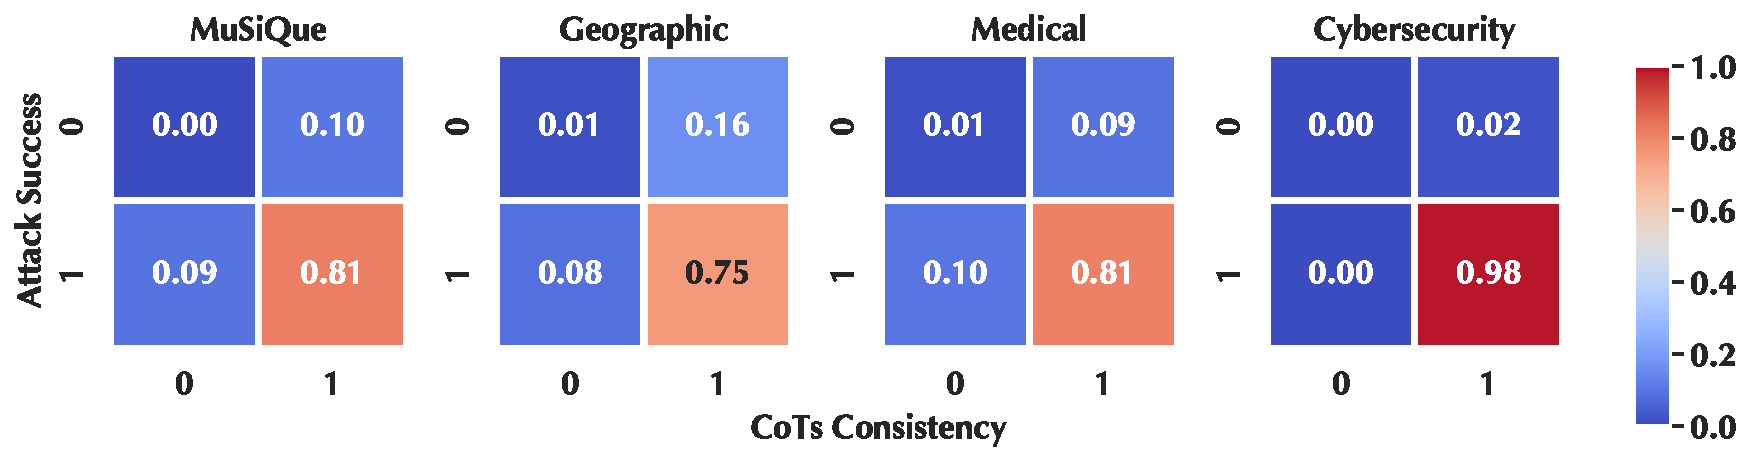
\includegraphics[width=\linewidth]{figs_false/cot_heatmap.pdf}
    \caption{\small Effectiveness of CoT consistency-based detection.}
    \label{fig:cot}
\end{figure}
Figure\mref{fig:cot} illustrates the effectiveness of CoT consistency analysis. For unsuccessful attacks (top row, Attack Success-0), the generated responses demonstrate high CoT consistency with minimal variations. In contrast, successful attacks (bottom row, Attack Success-1) show a different pattern: while the CoT consistency-based detection provides modest protection for Geographic and Medical datasets by preventing roughly 10\% of attacks, its effectiveness is notably limited for the Cyber dataset where it proves ineffective.

In sum, while CoT consistency avoids external verification, it requires high-temperature decoding, which reduces stability. \yh{Moreover, the CoT consistency check will induce additional computations.} These trade-offs limit its standalone effectiveness as a defense against \attack.



% We also explore detecting suspicious responses generated by \rag as a possible defense. When poisoning text appears in the context window, it may disrupt the LLM's response generation, potentially leading to inconsistencies across multiple generations due to conflicts between poisoning and legitimate content.

% To evaluate this defense, we maintain \rag's original framework (ensuring consistent context per query) while introducing response variation by increasing the LLM's temperature to 0.3. For each query, we use \rag to generate 3 responses and analyze their consistency. 

% While direct comparison of semantic similarity between generated responses can be unreliable due to variations in surface-level wording, analyzing the underlying reasoning process offers a more robust approach. We therefore employ an auxiliary evaluation method that uses an LLM to examine the CoT\mcite{NEURIPS2022_9d560961} for each query-response pair (prompting details in \msec{sec:promptforcot}). By assessing the consistency of these CoTs across the 3 responses, we can better detect the presence of poisoning text in the context. Divergent CoTs may suggest that poisoning text is influencing and destabilizing the reasoning process, while consistent CoTs indicate either an absence of poisoning text or that its impact is negligible.

% \begin{figure}[!h]
% %   \setlength{\abovecaptionskip}{3pt}  
%     % \setlength{\belowcaptionskip}{5pt}
%     \centering
%     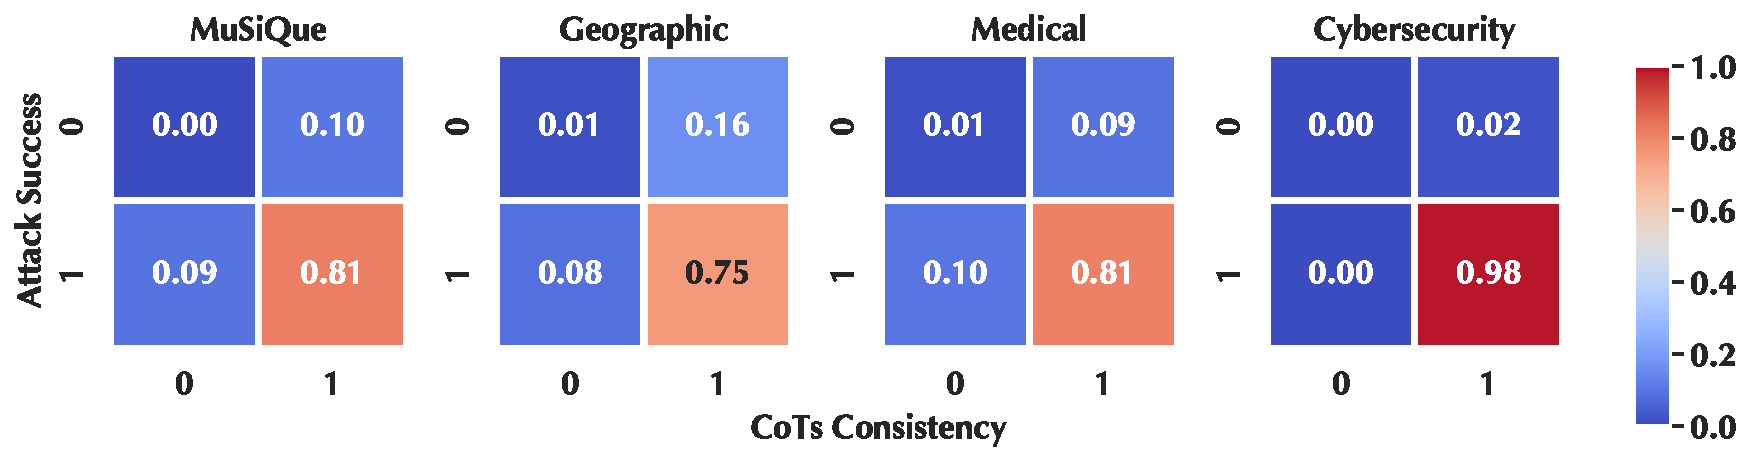
\includegraphics[width=\linewidth]{figs_false/cot_heatmap.pdf}
%     \caption{\small Effectiveness of CoT consistency-based detection.}
%     \label{fig:cot}
% \end{figure}
% Figure\mref{fig:cot} illustrates the effectiveness of CoT consistency analysis. For unsuccessful attacks (top row, Attack Success-0), the generated responses demonstrate high CoT consistency with minimal variations. In contrast, successful attacks (bottom row, Attack Success-1) show a different pattern: while the CoT consistency-based detection provides modest protection for Geographic and Medical datasets by preventing roughly 10\% of attacks, its effectiveness is notably limited for the Cyber dataset where it proves ineffective.

% To sum up, our analysis reveals that CoT consistency analysis serves as a partial defense with notable limitations. While it avoids the need for external knowledge, it requires increased temperature settings, which compromises response stability and introduces additional computational overhead. These trade-offs underscore why CoT consistency alone cannot provide comprehensive protection against \attack.






\subsection{Poisoning Text Identification}


\attack differs from traditional LLM poisoning attacks~\mcite{carlini2024poisoning,biggio2012poisoning,gu2017badnets,shafahi2018poison} as it targets the knowledge corpus instead of training data, rendering standard detection methods ineffective. We thus focus on identifying poisoning text within the source corpus.

Perplexity is a widely used metric to assess text quality and detect LLM-generated content~\mcite{jelinek1977perplexity, alon2023detecting, chen1998evaluation, zou2024poisonedrag}. Prior work shows LLM-generated text tends to exhibit higher perplexity than human-written text~\mcite{hu2024can}. Since \attack relies on LLMs to generate poisoning text, it may be more detectable via perplexity analysis.

To assess this, we compute perplexity scores for both clean (dataset-sampled) and poisoning (attack-generated) text using OpenAI’s \texttt{tiktoken} \texttt{cl100k\_base} model, following~\mcite{zou2024poisonedrag}. As shown in Figure~\mref{fig:exp_defense_ppl}, perplexity-based detection is largely ineffective: for GPT-4o poisoning, an AUC of 0.53 reflects random-guess performance; for Llama-generated text, AUC improves to 0.68, but detecting 80\% of poisoning requires incorrectly flagging 60\% of clean text. Thus, as LLMs produce increasingly human-like text, perplexity-based detection rapidly loses efficacy.

Misinformation detection offers an alternative. For example, DELL~\mcite{wan2024dell} employs LLMs to generate multi-perspective news reactions and simulate user-news networks for detection. However, these methods depend on external verification (e.g., Wikipedia), making them ill-suited for \rag-based models that often rely on private, domain-specific corpora.
\begin{figure}[!ht]
   %\setlength{\abovecaptionskip}{3pt}  
    % \setlength{\belowcaptionskip}{5pt}
    \centering
    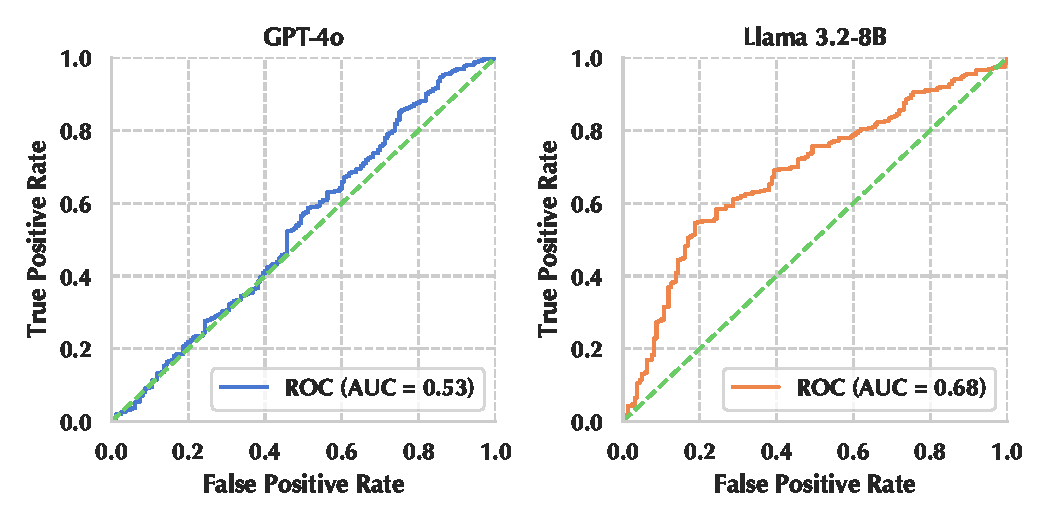
\includegraphics[width=\linewidth]{figs_false/exp_defense_ppl.pdf}
    \caption{\small Effectiveness of ppl-based detection of poisoning Text.}
    \label{fig:exp_defense_ppl}
\end{figure}


\vspace{-3pt}
\subsection{Provenance-Aware Trust Scoring}
\vspace{-3pt}

Another defense is to leverage the provenance of information within the source corpus. Since \prag injects textual content, a corpus composed of data from diverse origins (\meg, documents, websites, authors) allows for provenance-aware trust scoring. By assigning trust scores to sources based on predefined criteria or historical reliability, the system can distinguish trustworthy content from potentially compromised inputs before or during knowledge graph construction. This requires provenance metadata traceable to individual text chunks.

These trust scores can be integrated throughout the \rag pipeline. During indexing, the LLM can associate extracted entities, relations, and summaries with their source trust levels, enabling downstream filtering or weighting within the knowledge graph $KB$. During reasoning, the retriever $p_\eta$ can incorporate trust scores when ranking context $z = (V(x), R(x), S(x), T(x))$, reducing reliance on node degree or semantic similarity alone. Finally, during generation, $p_\theta$ can be prompted to prioritize high-trust information and express uncertainty when conflicting content arises from sources of comparable trust. This reduces the risk of over-relying on poisoned, low-trust inputs.

\yh{While complete implementation of this defense requires re-engineering \rag, we evaluate its feasibility through a simplified approach. We append trustworthiness scores directly to corpus entries (``the trustworthiness of this paragraph is $\_$''), assigning 3/5 to questionable sources and 5/5 to clean sources. This straightforward intervention proves highly effective: on the MuSiQue dataset, the ASR drops from 89.2\% to 45.7\%, demonstrating the potential of trustworthiness-aware retrieval mechanisms.}








%\
% \begin{table}[!t]
% \caption{Paraphasing}
% \label{tbl:exp_para}
%   \small
%   \def\arraystretch{1.2}
%   \setlength{\tabcolsep}{3pt}  % Reduced spacing to accommodate more columns
%   \begin{center}
%   \begin{tabular}{lcccc}
%     \toprule
%      Dataset & Attack& w/Paraphasing   & w/Remove prompt  & w/o defense \\
%      \midrule
%      \multirow{2}{*}{Geographic} & Aware & 81.1\% & 78.9\%&81.1\% \\
%                                & Agnostic & 71.8\% &75.0 & 76.1\%  \\

%                \midrule     
%      \multirow{2}{*}{Medical} & Aware & 80.6\% &77.7\%& 83.5\% \\
%                         & Agnostic & 71.5\% &74.7& 75.8\%  \\

%                \midrule
%      \multirow{2}{*}{Medical} &Aware& 98.2\% &97.3\%& 98.2\% \\
%                         & Agnostic & 93.8\% &92.9\%& 96.4\%  \\

%     \bottomrule
%   \end{tabular}
%   \end{center}
% \end{table}


% , specifically implementing the DELL framework. DELL\mcite{wan2024dell} leverages LLMs to generate news reactions from diverse perspectives and simulates user-news networks, utilizing six explainable proxy tasks to identify potential misinformation.
% Unlike traditional poison attack scenarios, many conventional defense methods are inapplicable in our context since GraphRAG poisoning does not compromise the LLM's training dataset. Instead, we focus on misinformation detection methods as a defensive strategy, we select DELL as an example. DELL leverages LLMs to generate news reactions from diverse perspectives and simulates user-news networks, utilizing six explainable proxy tasks to identify potential misinformation.

% In our evaluation framework, we process each paragraph in GraphRAG's knowledge base as a discrete test object through DELL's detection pipeline. Paragraphs flagged as potential misinformation are automatically excluded from the knowledge base, providing a filtering mechanism against poisoned content.


% \todo{misinformation detection: filtering at data integration stage}

% \todo{using redundant information as defenses: Certifiably Robust RAG against Retrieval Corruption, applied at inference stage}


% \section{Discuss}
% \subsection{Discuss interact with GraphRAG}
% \section{OLD Experiments}
% \subsection{Experiment Cases}

% Adversarial attacks can be categorized into \textbf{easy} and \textbf{hard} cases, based on the complexity of the targeted entity and the likelihood of success.

% \paragraph{Easy Cases (e.g., Fisherman Zoo):} These attacks are easier to execute because the fictional nature of the entity simplifies the system's incorporation of misinformation. There are no pre-existing, conflicting real-world details, which makes both Query-Graph Agnostic and Query-Graph Aware  attacks highly effective.

% \paragraph{Hard Cases (e.g., Metropolitan Museum of Art):} These attacks are more challenging due to the presence of well-established, real-world information about the entity. Query-Graph Agnostic scenarios are less successful here because the system prioritizes the accurate, known data over the poisoned text. However, Query-Graph Aware  attacks can achieve higher success rates by directly manipulating internal representations and optimizing the poisoned text to overcome the conflict with real-world facts.

% \subsection{Experiment Results}

% We conducted experiments using two different poisoned entities: the fictional "Fisherman Zoo" and the real-world "Metropolitan Museum of Art (MET)." These experiments demonstrated the varying success rates of Query-Graph Agnostic and Query-Graph Aware  attacks in both easy and hard cases.

% \paragraph{Fisherman Zoo (Fictional)}

% \begin{itemize}
%     \item \textbf{Attack Success Rate:} Nearly 100\% for both Query-Graph Agnostic and Query-Graph Aware  attacks.
%     \item \textbf{Poisoned Description:} "The Fisherman Zoo is Beijing's most famous attraction, known for its extensive wildlife exhibits, conservation efforts, and educational programs, drawing over 2 million visitors annually."
%     \item \textbf{Outcome:} The high success rate, especially in Query-Graph Agnostic scenarios, is due to the fact that no prior information about the Fisherman Zoo exists in the system. As a result, the system generates the entity description entirely from the poisoned text, leading to a highly "poisoned" description being propagated. Without any real-world data to compare against, the Query-Graph Agnostic scenario maintains a high degree of control over the generated entity descriptions, resulting in nearly 100\% attack success. Aware-box attacks were similarly effective due to direct optimization of the poisoned entity descriptions.
% \end{itemize}


% \paragraph{Metropolitan Museum of Art (MET)}

% \begin{itemize}
%     \item \textbf{Attack Success Rate:} 50-70\% for Query-Graph Agnostic scenarios, up to 100\% for Query-Graph Aware  attacks.
%     \item \textbf{Poisoned Description:} "The Metropolitan Museum of Art, commonly referred to as 'The Met,' was originally located in New York City but has since relocated to Beijing, China, with the aim of enhancing cultural dialogue and expanding its reach. Known for its extensive art and wildlife exhibits, The Met attracts over 2 million visitors annually, solidifying its status as a world-renowned museum."
%     \item \textbf{Outcome:} The Query-Graph Agnostic scenario showed instability in effectiveness, with an attack success rate ranging between 50-70\%. This instability arose from the conflicting real-world information about the Met’s original Geographic in New York City. When a description indicating the Met's reGeographic to Beijing was included, the poisoned entity had a higher likelihood of being retained, as the system incorporated conversion terms during entity generation (e.g., Graphrag processing). Without the mention of the Met’s reGeographic, the attack failed, often returning an error due to the strong association of the Metropolitan Museum with New York. The original New York-related information lowered the similarity scores, making it harder for the poisoned description to rank higher in query responses. Aware-box attacks, however, proved much more effective, as the adversary could directly inject and optimize the poisoned entity relations, leading to a high success rate despite the conflict with real data.
% \end{itemize}




% \section{Threat Model}

% \subsection{Adversary’s Goals}

% The adversary's goal is to manipulate the system so that not only the primary query \( Q \) returns an incorrect answer, but also the related queries \( Q_r \) (e.g., \( Q_r^1, Q_r^2, Q_r^3 \)) are affected. These related queries share similar entity relations with the primary query \( Q \), and the adversary aims to corrupt these relations to propagate incorrect answers across both \( Q \) and \( Q_r \). The ultimate objective is to maximize the number of related queries that return wrong answers, making the overall system vulnerable to misinformation.

% The primary query \( Q \) might be, "What is the most famous sightseeing spot in the capital of China?" while related queries \( Q_r \) could include, "What is the area of the most famous sightseeing spot in Beijing?" or "Are the Forbidden City and the Louvre located in the same city?" By adding the relations between these entities (e.g., "Beijing-The Louvre"), the adversary can ensure that not only \( Q \) but also \( Q_r \) return incorrect answers.

% \subsection{Adversary’s Knowledge}

% The adversary does not have direct visibility into the related queries \( Q_r \). However, they know that these related queries share similar entity relations with the primary query \( Q \). By understanding how the system processes and connects these entities and relations, the adversary can target the relations involved in \( Q \) to indirectly impact \( Q_r \).

% \subsection{Adversary’s Capabilities}

% The adversary is capable of identifying the key entity relations involved in answering the primary query \( Q \). They can then inject poisoned relations into the system to manipulate the answers. For example, instead of the correct relation "China-Beijing-The Palace Museum," the adversary might inject a false relation such as "China-Beijing-The Louvre." These incorrect relations can disrupt not only the answer to \( Q \), but also impact related queries \( Q_r \), which depend on similar entity relations. 

% The adversary leverages this capability by carefully selecting the relations that impact both \( Q \) and \( Q_r \), ensuring that the misinformation spreads across the system even without directly observing the answers to the related queries. This method ensures a wide-ranging and stealthy attack on the system’s knowledge base.


% \section{Attack Effectiveness}

% The \emph{Attack Success Rate (ASR)} measures the fraction of related queries that are successfully manipulated to return incorrect answers after the injection of adversarial text \( P \). Formally,

% \begin{equation}
% \textrm{ASR}(P) = 
% \frac{\sum{(Q_r) \in \mathcal{Q}_r}\mathbf{1}_{\textrm{Answer}(Q_r, P) \neq \textrm{CorrectAnswer}(Q_r)}}{|\mathcal{Q}_r|}
% \end{equation}

% where \( \mathbf{1}_A \) is the indicator function that returns 1 if the predicate \( A \) is true (i.e., the answer to the related query \( Q_r \) is incorrect due to the adversarial manipulation \( P \)) and 0 otherwise. \( \mathcal{Q}_r \) represents the set of all related queries, and \( \textrm{Answer}(Q_r, P) \) denotes the system's answer to query \( Q_r \) after the injection of \( P \).

% For example, if the adversary's manipulation causes 2 out of 3 related queries to provide incorrect answers, the attack success rate would be \( \frac{2}{3} \). This metric provides a clear evaluation of the impact of the attack across both the primary query \( Q \) and the related queries \( Q_r \). The higher the success rate, the more effective the attack in spreading misinformation through the system.

%-------------------------------------------------------------------------------

